% =====================================================================
% ICIP 2027 submission -- IEEE conference format, A4
%
% COMPILER: pdfLaTeX (recommended). XeLaTeX also still works.
%   Overleaf: Menu > Compiler > pdfLaTeX
%
% The font block below branches automatically:
%   pdfLaTeX -> T1 encoding + newtx (Times-compatible text and math)
%   XeLaTeX  -> fontspec + Times New Roman (or the four .ttf files)
% Only ONE branch is executed, so pdfLaTeX never sees fontspec.
% =====================================================================
\documentclass[conference,a4paper]{IEEEtran}

\usepackage{amsmath,amssymb,amsfonts}

\usepackage{iftex}
\ifPDFTeX
  % ---- pdfLaTeX path: Times-compatible Type1 fonts, clean text layer ----
  \usepackage[T1]{fontenc}
  \usepackage{newtxtext,newtxmath}
\else
  % ---- XeLaTeX / LuaLaTeX path ----
  \usepackage{fontspec}
  \IfFileExists{times.ttf}{%
    \setmainfont{times.ttf}[
      BoldFont=timesbd.ttf,
      ItalicFont=timesi.ttf,
      BoldItalicFont=timesbi.ttf,
      Ligatures=TeX]%
    \setsansfont{times.ttf}[
      BoldFont=timesbd.ttf,
      ItalicFont=timesi.ttf,
      BoldItalicFont=timesbi.ttf]%
    \setmonofont{times.ttf}[
      BoldFont=timesbd.ttf,
      ItalicFont=timesi.ttf,
      BoldItalicFont=timesbi.ttf]%
  }{%
    \IfFontExistsTF{Times New Roman}{%
      \setmainfont{Times New Roman}[Ligatures=TeX]%
      \setsansfont{Times New Roman}%
      \setmonofont{Times New Roman}%
    }{%
      \PackageError{ConferenceFont}{Times New Roman was not found}%
        {Upload times.ttf, timesbd.ttf, timesi.ttf and timesbi.ttf to the project, or install Times New Roman.}%
    }%
  }%
\fi

% ---- packages ----
\usepackage{cite}
\usepackage{graphicx}
\usepackage{textcomp}
\usepackage{xcolor}
\usepackage{url}
\usepackage{booktabs}
\usepackage{tikz}
\usetikzlibrary{arrows.meta}

% For a double-blind PDF, change the next line to \anonymousreviewtrue.
% If reviewers receive source files, remove identifying information from the
% source as well and follow the conference's anonymity policy.
\newif\ifanonymousreview
\anonymousreviewfalse

\begin{document}

% ---- every number below is generated from backend/*.json by
%      backend/scripts/export_paper_metrics.py - edit the code, not this file
% Generated 2026-10-31 05:31 UTC
% Source: backend/*.json - do not edit by hand

\newcommand{\CorpusMemories}{15}
\newcommand{\CorpusQuestions}{11}
\newcommand{\CorpusAnswerable}{9}
\newcommand{\CoreVanillaStaleCount}{4}
\newcommand{\CoreVanillaEvid}{0.963}
\newcommand{\CoreVanillaHit}{1.000}
\newcommand{\CoreVanillaMrr}{0.833}
\newcommand{\CoreVanillaStale}{0.364}
\newcommand{\CoreVanillaStaleRate}{0.089}
\newcommand{\CoreVanillaLeak}{0.022}
\newcommand{\CoreVanillaDup}{0.022}
\newcommand{\CoreVanillaLatency}{29}
\newcommand{\CoreHybridStaleCount}{2}
\newcommand{\CoreHybridEvid}{1.000}
\newcommand{\CoreHybridHit}{1.000}
\newcommand{\CoreHybridMrr}{0.944}
\newcommand{\CoreHybridStale}{0.182}
\newcommand{\CoreHybridStaleRate}{0.087}
\newcommand{\CoreHybridLeak}{0.022}
\newcommand{\CoreHybridDup}{0.022}
\newcommand{\CoreHybridLatency}{23}
\newcommand{\CoreGraphStaleCount}{2}
\newcommand{\CoreGraphEvid}{1.000}
\newcommand{\CoreGraphHit}{1.000}
\newcommand{\CoreGraphMrr}{0.944}
\newcommand{\CoreGraphStale}{0.182}
\newcommand{\CoreGraphStaleRate}{0.087}
\newcommand{\CoreGraphLeak}{0.022}
\newcommand{\CoreGraphDup}{0.022}
\newcommand{\CoreGraphLatency}{76}
\newcommand{\CoreAdaptiveStaleCount}{0}
\newcommand{\CoreAdaptiveEvid}{1.000}
\newcommand{\CoreAdaptiveHit}{1.000}
\newcommand{\CoreAdaptiveMrr}{1.000}
\newcommand{\CoreAdaptiveStale}{0.000}
\newcommand{\CoreAdaptiveStaleRate}{0.070}
\newcommand{\CoreAdaptiveLeak}{0.000}
\newcommand{\CoreAdaptiveDup}{0.000}
\newcommand{\CoreAdaptiveLatency}{51}
\newcommand{\CoreAdaptiveGraphStaleCount}{0}
\newcommand{\CoreAdaptiveGraphEvid}{1.000}
\newcommand{\CoreAdaptiveGraphHit}{1.000}
\newcommand{\CoreAdaptiveGraphMrr}{1.000}
\newcommand{\CoreAdaptiveGraphStale}{0.000}
\newcommand{\CoreAdaptiveGraphStaleRate}{0.070}
\newcommand{\CoreAdaptiveGraphLeak}{0.000}
\newcommand{\CoreAdaptiveGraphDup}{0.000}
\newcommand{\CoreAdaptiveGraphLatency}{100}
\newcommand{\PersonaQueries}{30}
\newcommand{\PersonaUniqueQueries}{30}
\newcommand{\PersonaAnswerable}{25}
\newcommand{\PersonaCount}{5}
\newcommand{\PersonaVanillaMrr}{0.880}
\newcommand{\PersonaVanillaStale}{0.333}
\newcommand{\PersonaVanillaLeak}{0.062}
\newcommand{\PersonaHybridMrr}{0.940}
\newcommand{\PersonaHybridStale}{0.233}
\newcommand{\PersonaHybridLeak}{0.045}
\newcommand{\PersonaGraphMrr}{0.940}
\newcommand{\PersonaGraphStale}{0.233}
\newcommand{\PersonaGraphLeak}{0.045}
\newcommand{\PersonaAdaptiveMrr}{0.960}
\newcommand{\PersonaAdaptiveStale}{0.067}
\newcommand{\PersonaAdaptiveLeak}{0.000}
\newcommand{\PersonaAdaptiveGraphMrr}{0.960}
\newcommand{\PersonaAdaptiveGraphStale}{0.067}
\newcommand{\PersonaAdaptiveGraphLeak}{0.000}
\newcommand{\ScaleMaxDecoys}{100}
\newcommand{\ScaleMemories}{115}
\newcommand{\ScaleFirstMemories}{15}
\newcommand{\ScaleHybridEvid}{1.000}
\newcommand{\ScaleAdaptiveEvid}{1.000}
\newcommand{\ScaleHybridMrr}{0.889}
\newcommand{\ScaleHybridDup}{0.234}
\newcommand{\ScaleHybridStale}{0.273}
\newcommand{\ScaleAdaptiveMrr}{1.000}
\newcommand{\ScaleAdaptiveDup}{0.000}
\newcommand{\ScaleAdaptiveStale}{0.000}
\newcommand{\AblHybridMrr}{0.944}
\newcommand{\AblHybridStale}{0.182}
\newcommand{\AblHybridDup}{0.022}
\newcommand{\AblHybridLeak}{0.022}
\newcommand{\AblTemporalMrr}{1.000}
\newcommand{\AblTemporalStale}{0.091}
\newcommand{\AblTemporalDup}{0.022}
\newcommand{\AblTemporalLeak}{0.022}
\newcommand{\AblContradictionMrr}{1.000}
\newcommand{\AblContradictionStale}{0.091}
\newcommand{\AblContradictionDup}{0.022}
\newcommand{\AblContradictionLeak}{0.043}
\newcommand{\AblConsolidationMrr}{1.000}
\newcommand{\AblConsolidationStale}{0.091}
\newcommand{\AblConsolidationDup}{0.000}
\newcommand{\AblConsolidationLeak}{0.046}
\newcommand{\AblForgettingMrr}{1.000}
\newcommand{\AblForgettingStale}{0.000}
\newcommand{\AblForgettingDup}{0.000}
\newcommand{\AblForgettingLeak}{0.000}
\newcommand{\AblAllMrr}{1.000}
\newcommand{\AblAllStale}{0.000}
\newcommand{\AblAllDup}{0.000}
\newcommand{\AblAllLeak}{0.000}
\newcommand{\CoreDeltaMrr}{+0.056}
\newcommand{\CoreDeltaMrrLo}{+0.000}
\newcommand{\CoreDeltaMrrHi}{+0.167}
\newcommand{\CoreDeltaStale}{-0.182}
\newcommand{\CoreDeltaStaleLo}{-0.455}
\newcommand{\CoreDeltaStaleHi}{+0.000}
\newcommand{\PersonaDeltaMrr}{+0.020}
\newcommand{\PersonaDeltaMrrLo}{+0.000}
\newcommand{\PersonaDeltaMrrHi}{+0.060}
\newcommand{\PersonaDeltaStale}{-0.200}
\newcommand{\PersonaDeltaStaleLo}{-0.280}
\newcommand{\PersonaDeltaStaleHi}{-0.133}
\newcommand{\TestPassed}{29}
\newcommand{\TestSkipped}{0}
\newcommand{\TestFailed}{0}

% generated from conflict_accuracy{,_holdout}.json
\newcommand{\NliDevPairs}{21}
\newcommand{\NliDevPositives}{10}
\newcommand{\NliDevPrecision}{1.000}
\newcommand{\NliDevRecall}{1.000}
\newcommand{\NliDevFone}{1.000}
\newcommand{\NliDevTp}{10}
\newcommand{\NliDevFp}{0}
\newcommand{\NliDevFn}{0}
\newcommand{\NliDevValueChangeGold}{7}
\newcommand{\NliDevValueChangeDetected}{7}
\newcommand{\NliDevNegationGold}{3}
\newcommand{\NliDevNegationDetected}{3}
\newcommand{\NliHoldPairs}{12}
\newcommand{\NliHoldPositives}{6}
\newcommand{\NliHoldPrecision}{0.857}
\newcommand{\NliHoldRecall}{1.000}
\newcommand{\NliHoldFone}{0.923}
\newcommand{\NliHoldTp}{6}
\newcommand{\NliHoldFp}{1}
\newcommand{\NliHoldFn}{0}
\newcommand{\NliHoldValueChangeGold}{3}
\newcommand{\NliHoldValueChangeDetected}{3}
\newcommand{\NliHoldNegationGold}{3}
\newcommand{\NliHoldNegationDetected}{3}
\newcommand{\NliPrecision}{1.000}
\newcommand{\NliRecall}{1.000}
\newcommand{\NliFone}{1.000}
\newcommand{\NliTp}{10}
\newcommand{\NliFp}{0}
\newcommand{\NliFn}{0}


\title{Adaptive Temporal Personal Knowledge Graph with Memory Consolidation and Contradiction-Aware Retrieval-Augmented Generation}

\ifanonymousreview
\author{\IEEEauthorblockN{Anonymous Authors}}
\else
\author{%
\IEEEauthorblockN{Maria Immanuel L}
\IEEEauthorblockA{\textit{School of Computing}\\
\textit{Vel Tech Rangarajan Dr Sagunthala}\\
\textit{R\&D Institute of Science}\\
\textit{and Technology}\\
Chennai, India\\
\texttt{vtu24334@veltech.edu.in}}
\and
\IEEEauthorblockN{Vigneshwaran S}
\IEEEauthorblockA{\textit{School of Computing}\\
\textit{Vel Tech Rangarajan Dr Sagunthala}\\
\textit{R\&D Institute of Science}\\
\textit{and Technology}\\
Chennai, India\\
\texttt{vtu24372@veltech.edu.in}}
\and
\IEEEauthorblockN{Dr. P S Anu Rakhi}
\IEEEauthorblockA{\textit{School of Computing}\\
\textit{Assistant Professor}\\
\textit{Vel Tech Rangarajan Dr Sagunthala}\\
\textit{R\&D Institute of Science}\\
\textit{and Technology}\\
Chennai, India\\
\texttt{anurakhips@veltech.edu.in}}
}
\fi

\maketitle

\begin{abstract}
Personal retrieval systems can encounter outdated, conflicting, duplicate, or deliberately removed memories. We present SecondBrain, an architecture combining importance scoring, temporal facts, conflict-aware ranking, consolidation, knowledge-gap detection, and retrieval-level forgetting. We independently reran the repository benchmarks using term frequency--inverse document frequency (TF-IDF) retrieval, an ONNX natural language inference model, and spaCy parsing. On \CorpusMemories{} synthetic memories and \CorpusQuestions{} questions, mean reciprocal rank (MRR) over \CorpusAnswerable{} answerable questions was \CoreVanillaMrr{} for TF-IDF, \CoreHybridMrr{} for hybrid and graph modes, and \CoreAdaptiveMrr{} for adaptive retrieval; stale or forbidden results appeared at rank one for \CoreVanillaStaleCount/11, \CoreHybridStaleCount/11, \CoreGraphStaleCount/11, and \CoreAdaptiveStaleCount/11 questions. In a separately isolated rerun of five synthetic personas (30 queries, \PersonaAnswerable{} answerable), MRR was \PersonaVanillaMrr{}, \PersonaHybridMrr{}, \PersonaGraphMrr{}, and \PersonaAdaptiveMrr{}, respectively, and stale@1 fell from \PersonaHybridStale{} to \PersonaAdaptiveStale{}. Scaling the distractor pool from \CorpusMemories{} to \ScaleMemories{} memories leaves adaptive MRR at \ScaleAdaptiveMrr{} while hybrid degrades to \ScaleHybridMrr{} and its duplicate rate rises to \ScaleHybridDup{}. Results concern retrieval, not generated answers, and establish neither real-world generalisation nor permanent erasure.
\end{abstract}

\begin{IEEEkeywords}
personal knowledge management, retrieval-augmented generation, temporal knowledge graphs, contradiction detection, memory consolidation, retrieval-level forgetting
\end{IEEEkeywords}

\section{Introduction}
Retrieval-augmented generation technology (RAG) uses retrieved evidence to support responses generated by language models [1], [2]. In the context of a personal knowledge base, the stored information can change over time, be duplicated, contradict newer records, or be explicitly removed. Thus, even if the response to the question is supported by the retrieved document, it can still be irrelevant for the user's current state.

For example, consider an earlier note from January about learning Python and a later note about a switch of focus to Java. The retriever may rank the earlier record as the most relevant even though it is outdated. In other cases the historical records are entirely appropriate, for instance when the query concerns a person's past studies.

We examine whether temporal validity, conflict-aware ranking of records, consolidation of information, and explicit exclusion can improve the ranking of retrieved evidence. The paper reports an experiment comparing four retrieval methods, together with evaluations through ablation studies.

\section{Related Work}
\subsection{Retrieval and Graph-Based Methods}
Dense passage retrieval \cite{b3} and probabilistic lexical ranking \cite{b4} are established approaches, while vector-store designs are surveyed in \cite{b5}. Graph-based retrieval \cite{b6,b7}, knowledge-graph representations \cite{b8}, and temporal knowledge graphs \cite{b9} motivate structured and time-aware evidence. Our TF-IDF vector baseline is lexical and should not be interpreted as a neural dense-embedding comparison.

\subsection{Agent Memory, Removal, and Consistency}
Agent-memory surveys discuss persistence, memory mechanisms, and lifelong adaptation \cite{b10,b11,b12}. Machine unlearning concerns the influence of training data on model parameters \cite{b13}; retrieval-level exclusion is different and makes no claim about model-parameter unlearning. Self-reflection \cite{b14}, corrective retrieval \cite{b15}, retrieval optimisation \cite{b16}, and certainty estimation \cite{b17} address related reliability problems. Outdated evidence can nevertheless remain consistent with a source passage.

LongMemEval tests knowledge updates and temporal reasoning \cite{b22}, HoH studies outdated RAG evidence \cite{b23}, and STALE evaluates implicit conflicts in personal agent memory \cite{b24}. The contribution here is a particular set of retrieval-level diagnostics, not the first benchmark of changing knowledge.

\section{System Architecture and Methodology}
The system uses a FastAPI backend with SQLite, an optional vector store, and an Electron/React client. Optional components include sentence embeddings \cite{b18}, approximate nearest-neighbour indexing \cite{b19}, language models \cite{b20}, and speech recognition \cite{b21}. The experiments below used deterministic lexical TF-IDF retrieval, not neural embeddings, and did not evaluate generation. The research layer is switchable and stores derived records keyed by memory identifier. Capture and normalisation precede scoring, temporal extraction, conflict handling, consolidation, retrieval, and optional generation. Fig.~\ref{fig:architecture} is an architectural overview rather than evidence that every optional component was active.

\begin{figure}[t]
\centering
% Scalable vector artwork: no external image or fixed DPI is required.
\resizebox{0.98\columnwidth}{!}{%
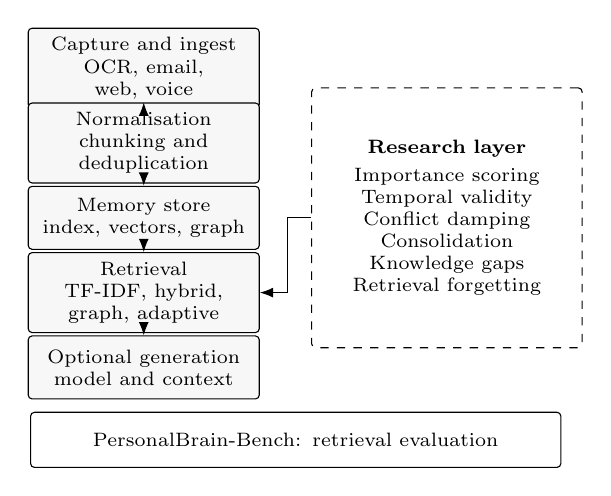
\begin{tikzpicture}[
  >=Latex,
  stage/.style={draw, rounded corners=1.4pt, fill=black!3,
    text width=27mm, minimum height=8mm, align=center, font=\scriptsize},
  layer/.style={draw, dashed, rounded corners=1.4pt, text width=32mm,
    minimum height=33mm, align=center, font=\scriptsize},
  bench/.style={draw, rounded corners=1.4pt, text width=65mm,
    minimum height=7mm, align=center, font=\scriptsize}
]
\node[stage] (capture) at (0,0) {Capture and ingest\\\scriptsize OCR, email, web, voice};
\node[stage] (normal) at (0,-0.95) {Normalisation\\\scriptsize chunking and deduplication};
\node[stage] (store) at (0,-1.90) {Memory store\\\scriptsize index, vectors, graph};
\node[stage] (retrieve) at (0,-2.85) {Retrieval\\\scriptsize TF-IDF, hybrid, graph, adaptive};
\node[stage] (generate) at (0,-3.80) {Optional generation\\\scriptsize model and context};
\node[layer] (research) at (3.85,-1.90) {\textbf{Research layer}\\[2pt]
Importance scoring\\
Temporal validity\\
Conflict damping\\
Consolidation\\
Knowledge gaps\\
Retrieval forgetting};
\node[bench] (benchmark) at (1.93,-4.72) {PersonalBrain-Bench: retrieval evaluation};
\draw[->] (capture) -- (normal);
\draw[->] (normal) -- (store);
\draw[->] (store) -- (retrieve);
\draw[->] (retrieve) -- (generate);
\draw[->] (research.west) -- ++(-0.30,0) |- (retrieve.east);
\end{tikzpicture}%
}
\caption{System architecture. The research layer annotates memory records or modifies retrieval. The benchmark evaluates retrieved items; generated answers were not evaluated. The diagram was produced using AI-generated TikZ code (see Acknowledgment).}
\label{fig:architecture}
\end{figure}

\begin{table}[t]
\caption{Adopted Techniques and Their Roles}
\label{tab:adopted}
\centering
\footnotesize
\begin{tabular}{@{}p{0.35\columnwidth}p{0.57\columnwidth}@{}}
\toprule
\textbf{Technique} & \textbf{Status and role} \\
\midrule
Vector and lexical fusion & Adopted; used for the hybrid comparison. \\
Knowledge graphs & Adopted; populated per corpus, used by the graph mode. \\
NLI and dependency parsing & Adopted tools for conflict and predicate handling. \\
Temporal validity & Adopted concept; facts are closed rather than erased. \\
Eight-term scoring & Proposed scoring configuration and audit record. \\
Conflict damping & Proposed integration for ranking, not deletion. \\
Forgetting and consolidation & Proposed retrieval exclusion and duplicate handling. \\
PersonalBrain-Bench & Proposed small diagnostic evaluation suite. \\
\bottomrule
\end{tabular}
\end{table}

\section{Proposed Method}
\subsection{Adaptive Memory Scoring}
The memory score combines relevance $R$, frequency $F$, recency $T$, graph connectivity $G$, user confirmation $U$, predicted utility $P$, redundancy $D$, and conflict $C$. The implementation uses bounded heuristic components and clips the final score:
\begin{equation}
\begin{aligned}
S ={}& 0.30R + 0.08F + 0.22T + 0.15G \\
     &+ 0.15U + 0.10P - 0.18D - 0.25C, \\
M ={}& \min\bigl(1.5,\max(0,S)\bigr).
\end{aligned}
\label{eq:score}
\end{equation}
The last two terms are penalties. Recency is $T=2^{-\Delta t/45}$, with $\Delta t$ in days. The meaning of relevance and future usefulness is based on term-based assumptions, not learned predictions. Given that the component limits are $[0,1]$, the respective weights restrict the real score to the range $[0,1]$ despite the higher clipping limit.

\subsection{Temporal Personal Knowledge Graph}
Facts are represented as subject--predicate--object statements that carry their own validity intervals $[t_{\mathrm{from}}, t_{\mathrm{to}})$. For stateful predicates, any newer value for the same subject and predicate closes the earlier fact instead of deleting it. In predicate canonicalization, rules are intertwined with the dependency parsing of spaCy, where verb lemmata and grammatical functions make it possible to group phrases such as learning and focusing into one state class. In the reruns, the model used was \texttt{en\_core\_web\_sm} 3.8.0. Historical-query accuracy and multi-valued predicate treatment call for special validation.

\subsection{Contradiction-Aware Ranking}
\label{sec:conflict}
Temporal supersession, negation and value changes are treated as potential conflicts. Four signals are combined: closed temporal facts, one-sided lexical negation over lexically close memories, typed value slots (a calendar date, a quantity with its unit, or a named entity) that differ between two memories about the same topic, and an INT8 DistilBERT natural language inference (NLI) model in ONNX Runtime. A pair is a conflict when the contradiction probability reaches 0.55 in \emph{both} premise orders; requiring both orders rather than the maximum removes topical pairs in which one direction happens to look contradictory. Two memories that both carry a restriction marker are never separated by the NLI signal alone, because a paraphrase such as ``never captures outside sessions'' and ``captures only inside sessions'' is read as a contradiction by the model.

For conflict severity $s\in[0,1]$, the damping factor is $1-0.7s$. It can be applied to a fused-rank prior $1/(1+i)$, where $i$ is a zero-based rank. Damping may reorder results and therefore does not guarantee that the original order is preserved.

The detector is evaluated on two author-annotated synthetic pair sets. The \NliDevPairs{}-pair development set (\NliDevPositives{} positive) was used while the rules were written, so its score is optimistic by construction: \NliDevTp{} of \NliDevPositives{} positives are found with \NliDevFp{} false positives on the \NliDevPairs{} pairs, precision \NliDevPrecision{}, recall \NliDevRecall{}, F1 \NliDevFone{}; value changes are detected \NliDevValueChangeDetected{}/\NliDevValueChangeGold{} and negations \NliDevNegationDetected{}/\NliDevNegationGold{}. A second \NliHoldPairs{}-pair set was written from unrelated domains and kept separate from rule design; it gives precision \NliHoldPrecision{}, recall \NliHoldRecall{}, F1 \NliHoldFone{}, with \NliHoldFp{} false positive. That false positive is a paraphrase that reorders a temporal boundary: ``avoids caffeine after 6\,pm'' against ``keeps caffeine intake to before 6\,pm''. Neither set is large or independently annotated, so these figures bound the detector on authored diagnostics rather than measure general detection performance.

\subsection{Memory Consolidation}
Memories that are almost identical are grouped based on cosine similarity calculated from term frequency counters. A representative is chosen through importance and length metric, but identifiers of the members are saved for the sake of traceability. The retrieval deduplication utilizes 0.78 as a cut-off point. The source explains that calibration is taking place in a benchmark corpus, hence a separate calibration split is not created. The v1 duplicate metric utilizes the same similarity algorithm but with a stricter threshold of 0.90. The absence of duplicate records, however, does not establish uniqueness semantically or prevent the merging of different records.

\subsection{Knowledge-Gap Detection}
The gap detector estimates a concept's depth from four signals: mention frequency, whether the concept is explained in the user's own notes, recurrence, and graph connectivity. It computes a gap score as
\begin{equation}
\begin{aligned}
\mathrm{gap} ={}& \mathrm{exposure}\,(1-\mathrm{depth}) \\
 &\times(1-0.5\,\mathrm{connectivity}).
\end{aligned}
\label{eq:gap}
\end{equation}
Here exposure is the mention count capped at 12 and normalised, connectivity is the normalised degree of the concept, and depth combines the explanation, subject and recurrence signals. No ground-truth validation of the gap predictions was performed, so the detector is reported as a heuristic rather than as a validated measure.

\subsection{Retrieval-Level Forgetting}
Soft forgetting destroys the memory of a tombstone, attempts to remove the text index reference, executes vector and graph deletion, and disconnects corresponding facts. The process of restoration annihilates the tombstone and reconstructs the text index, but it does not reconstruct all vectors, graphs, and derived data. Retrieval-level exclusion is reversible and does not prove permanent erasure from backups, logs, other copies, or model parameters. Zero observed leaks on these queries is not a universal privacy guarantee.

\subsection{PersonalBrain-Bench}
PersonalBrain-Bench v1 contains synthetic factual, temporal, contradiction, multi-hop, duplicate, gap and forgetting questions. A second suite defines five synthetic personas in software, machine-learning research, product operations, university academics, and health informatics; these are templates, not recruited participants.

\section{Experimental Setup}
\subsection{Corpus and Compared Systems}
The v1 corpus has 15 synthetic memories spanning 240 days and 11 questions, nine answerable. It includes a state change, a changed deadline, near-duplicates, multi-hop evidence, a forgotten note, and concept mentions. The five-persona suite has 11 memories and six queries per persona: 30 queries in total, of which 25 have gold memories. The remaining forgetting queries have no gold and are excluded from Hit@5 and MRR, not from stale@1 or leakage.

The four modes are TF-IDF vector, hybrid, graph-augmented, and adaptive. Vanilla retrieves TF-IDF candidates; hybrid fuses TF-IDF and keyword candidates with 0.7/0.3 weights and a recency bonus. The graph mode seeds from concepts named in the query, expands one predicate hop in the knowledge graph, weights seeds by inverse document frequency, and fuses the result with the lexical prior. Adaptive adds the research-layer operations to hybrid retrieval rather than that graph pass. Ingestion materialises every memory into the graph, so the graphs used here contain nodes and edges; graph and hybrid nevertheless converge on the metrics below because the corpus is small enough for both to return every gold item. Baselines and adaptive also do not share the same forgetting policy; the leak comparison is not an equal-deletion-policy ranking test.

\subsection{Metrics and Reproducibility}
Hit@5 is the fraction of answerable questions with a gold item in the first five results; MRR averages the reciprocal rank of the first gold item. They use nine v1 and 25 v2 answerable questions, respectively. These retrieval metrics do not show whether a multi-hop answer has all required evidence or whether a generated answer is correct.

Stale@1 uses all queries and counts a top result in that question's predefined forbidden set, which may include a forgotten item; it is not an independent general measure of temporal correctness. V1 leakage is the number of forgotten returned items divided by all returned items; v2 averages the per-query leak fraction. V1 duplicate rate divides the count of within-query pairs with term-frequency cosine at least 0.90 by the number of returned items. V2 instead averages within-query duplicate-pair fractions using token-set Jaccard similarity at 0.78. Rates are therefore not directly comparable across suites.

The four repository runners were executed on fresh SQLite databases at $k=5$ with TF-IDF retrieval, ONNX NLI, and spaCy parsing. Their non-latency aggregate metrics matched the committed artifacts. Each persona is ingested into a fresh database and its derived state is removed before the next persona starts, so Table~\ref{tab:multi} pools outcomes from five isolated runs. Core and isolated-persona reruns were repeated with matching non-latency outcomes. Environment details appear in Section~\ref{sec:verification}.

\section{Results and Comparative Analysis}
\subsection{Core-Corpus Results}
\begin{table}[t]
\caption{Reproduced Core-Corpus Retrieval Results}
\label{tab:core}
\centering
\footnotesize
\setlength{\tabcolsep}{3pt}
\begin{tabular}{@{}lccccc@{}}
\toprule
\textbf{System} & \textbf{Hit@5} & \textbf{MRR} & \textbf{Stale@1} & \textbf{Leak} & \textbf{Dup.} \\
\midrule
TF-IDF vector & 1.000 & 0.833 & 0.364 & 0.022 & 0.022 \\
Hybrid & 1.000 & 0.944 & 0.182 & 0.022 & 0.022 \\
Graph-aug. & 1.000 & 0.944 & 0.182 & 0.022 & 0.022 \\
Adaptive & 1.000 & 1.000 & 0.000 & 0.000 & 0.000 \\
Adaptive+graph & 1.000 & 1.000 & 0.000 & 0.000 & 0.000 \\
\bottomrule
\end{tabular}
\par\vspace{2pt}
\raggedright\scriptsize Hit@5 and MRR use \CorpusAnswerable{} answerable questions; stale@1 uses all \CorpusQuestions{} (\CoreVanillaStaleCount, \CoreHybridStaleCount, \CoreGraphStaleCount and \CoreAdaptiveStaleCount). The systems returned 45, 46, 46, 43 and 43 items, respectively.
\end{table}


Hit@5 is 1.000 for every configuration, while MRR and stale@1 differ. Each benchmark run builds a knowledge graph over the corpus (119 nodes, 147 edges, mean degree 2.47, every memory connected). The adaptive mode's zero stale@1 does not mean that no forbidden item was retrieved: its aggregate staleness rate over all returned items is \CoreAdaptiveStaleRate{}, so forbidden results appear below rank one even when they never take it. The zero duplicate and leak rates are limited to the stated metrics and test cases.

\begin{table}[t]
\caption{Reproduced MRR by Question Category}
\label{tab:category}
\centering
\footnotesize
\setlength{\tabcolsep}{4pt}
\begin{tabular}{@{}lcccc@{}}
\toprule
\textbf{Category} & \textbf{$n$} & \textbf{Hybrid} & \textbf{Adaptive} & $\boldsymbol{\Delta}$ \\
\midrule
Factual & 3 & 1.000 & 1.000 & $+0.000$ \\
Temporal & 2 & 0.750 & 1.000 & $+0.250$ \\
Contradiction & 2 & 1.000 & 1.000 & $+0.000$ \\
Multi hop & 1 & 1.000 & 1.000 & $+0.000$ \\
Duplicate & 1 & 1.000 & 1.000 & $+0.000$ \\
\bottomrule
\end{tabular}
\par\vspace{2pt}
\raggedright\scriptsize $\Delta$ is adaptive minus hybrid. The two no-gold questions are omitted.
\end{table}


The core script reports elapsed time over all \CorpusQuestions{} queries, not per-query latency. One run recorded \CoreVanillaLatency\,ms (TF-IDF), \CoreHybridLatency\,ms (hybrid), \CoreGraphLatency\,ms (graph-augmented) and \CoreAdaptiveLatency\,ms (adaptive); these are uncontrolled, environment-specific diagnostic timings rather than measurements.

\subsection{Five-Persona Results and Statistical Reporting}
\begin{table}[t]
\caption{Isolated Five-Persona Results}
\label{tab:multi}
\centering
\footnotesize
\setlength{\tabcolsep}{4pt}
\begin{tabular}{@{}lcccc@{}}
\toprule
\textbf{System} & \textbf{Hit@5} & \textbf{MRR} & \textbf{Stale@1} & \textbf{Leak} \\
\midrule
TF-IDF vector & 1.000 & 0.880 & 0.333 & 0.062 \\
Hybrid & 1.000 & 0.940 & 0.233 & 0.045 \\
Graph-aug. & 1.000 & 0.940 & 0.233 & 0.045 \\
Adaptive & 1.000 & 0.960 & 0.067 & 0.000 \\
Adaptive+graph & 1.000 & 0.960 & 0.067 & 0.000 \\
\bottomrule
\end{tabular}
\par\vspace{2pt}
\raggedright\scriptsize \PersonaCount{} isolated synthetic personas: MRR/Hit@5 over \PersonaAnswerable{} answerable queries; stale@1 over \PersonaQueries{}. Leak is the mean per-query fraction. Graph and hybrid coincide because both place every gold item inside the top five.
\end{table}


Adaptive matches hybrid on MRR (\PersonaAdaptiveMrr{} versus \PersonaHybridMrr{}) while reducing stale@1 from \PersonaHybridStale{} to \PersonaAdaptiveStale{} and eliminating forgotten-item leakage. Each persona is evaluated in a fresh database and the runner purges derived state -- temporal facts, conflicts, scores, tombstones and graph rows -- between personas, so no persona inherits another's annotations.

The suite contains five synthetic personas, not real users, and six queries share each persona, so query-level tests are not independent. We therefore resample personas rather than queries (cluster bootstrap, 10{,}000 resamples) and report intervals rather than $p$-values. Against hybrid the adaptive layer changes MRR by $\PersonaDeltaMrr$ with a 95\% interval of $[\PersonaDeltaMrrLo, \PersonaDeltaMrrHi]$ -- no evidence of an MRR effect -- but reduces stale@1 by $\PersonaDeltaStale$ $[\PersonaDeltaStaleLo, \PersonaDeltaStaleHi]$, an interval that excludes zero (Table~\ref{tab:bootstrap}). The honest reading is that the research layer improves the validity of the top-ranked result, not the depth of the ranking.

\begin{table}[t]
\caption{Paired Bootstrap of Adaptive Against Each Baseline}
\label{tab:bootstrap}
\centering
\scriptsize
\setlength{\tabcolsep}{2pt}
\begin{tabular}{@{}llcccc@{}}
\toprule
\textbf{Scope} & \textbf{Comparison} & $\boldsymbol{\Delta}$\textbf{MRR} & \textbf{95\% CI} & $\boldsymbol{\Delta}$\textbf{St.@1} & \textbf{95\% CI} \\
\midrule
Core & vs TF-IDF & $+0.167$ & $[+0.000, +0.333]$ & $-0.364$ & $[-0.636, -0.091]$ \\
Core & vs hybrid & $+0.056$ & $[+0.000, +0.167]$ & $-0.182$ & $[-0.455, +0.000]$ \\
Core & vs graph & $+0.056$ & $[+0.000, +0.167]$ & $-0.182$ & $[-0.455, +0.000]$ \\
Core & graph+ad. vs ad. & $+0.000$ & $[+0.000, +0.000]$ & $+0.000$ & $[+0.000, +0.000]$ \\
\midrule
Personas & vs TF-IDF & $+0.080$ & $[+0.020, +0.133]$ & $-0.240$ & $[-0.320, -0.150]$ \\
Personas & vs hybrid & $+0.020$ & $[+0.000, +0.060]$ & $-0.200$ & $[-0.280, -0.133]$ \\
Personas & vs graph & $+0.020$ & $[+0.000, +0.060]$ & $-0.200$ & $[-0.280, -0.133]$ \\
\bottomrule
\end{tabular}
\par\vspace{2pt}
\raggedright\scriptsize St.@1 is stale@1. Persona intervals use a cluster bootstrap over personas; core intervals resample questions.
\end{table}


\subsection{Distractor Scaling}
\label{sec:scaling}
The core corpus is small enough that Hit@5 saturates at 1.000 for every system, which hides any difference between retrievers. To test whether the research layer survives a harder candidate pool we hold the questions fixed and add topically similar distractor memories that never contain a gold or forbidden item. Table~\ref{tab:scaling} reports the result at \ScaleMemories{} memories. Adaptive MRR stays at \ScaleAdaptiveMrr{} while hybrid drops to \ScaleHybridMrr{}, and the separation widens on every validity metric: adaptive holds stale@1 at \ScaleAdaptiveStale{} while hybrid rises to \ScaleHybridStale{}, and hybrid's duplicate rate climbs to \ScaleHybridDup{} while adaptive stays at zero. Both systems keep evidence recall at \ScaleHybridEvid{}, so the loss is rank position, not recall of the required evidence. The research layer therefore does more work as the candidate pool grows: the same questions become no harder for adaptive while hybrid loses ranks and admits stale and duplicate items.

\begin{table}[t]
\caption{Distractor Scaling: Questions Fixed, Pool Grown}
\label{tab:scaling}
\centering
\footnotesize
\setlength{\tabcolsep}{3.5pt}
\begin{tabular}{@{}llcccccc@{}}
\toprule
\textbf{Pool} & \textbf{System} & \textbf{Hit@5} & \textbf{MRR} & \textbf{Evid.} & \textbf{Stale@1} & \textbf{Dup.} & \textbf{Leak} \\
\midrule
15 mem. & Hybrid & 1.000 & 0.944 & 1.000 & 0.182 & 0.022 & 0.022 \\
 & Graph-aug. & 1.000 & 0.944 & 1.000 & 0.182 & 0.022 & 0.022 \\
 & Adaptive & 1.000 & 1.000 & 1.000 & 0.000 & 0.000 & 0.000 \\
40 mem. & Hybrid & 1.000 & 0.944 & 1.000 & 0.182 & 0.170 & 0.021 \\
 & Graph-aug. & 1.000 & 0.944 & 1.000 & 0.182 & 0.192 & 0.021 \\
 & Adaptive & 1.000 & 1.000 & 1.000 & 0.000 & 0.000 & 0.000 \\
65 mem. & Hybrid & 1.000 & 0.944 & 1.000 & 0.182 & 0.192 & 0.021 \\
 & Graph-aug. & 1.000 & 0.944 & 1.000 & 0.182 & 0.213 & 0.021 \\
 & Adaptive & 1.000 & 1.000 & 1.000 & 0.000 & 0.000 & 0.000 \\
115 mem. & Hybrid & 1.000 & 0.889 & 1.000 & 0.273 & 0.234 & 0.021 \\
 & Graph-aug. & 1.000 & 0.889 & 1.000 & 0.273 & 0.255 & 0.021 \\
 & Adaptive & 1.000 & 1.000 & 1.000 & 0.000 & 0.000 & 0.000 \\
\bottomrule
\end{tabular}
\par\vspace{2pt}
\raggedright\scriptsize Evidence recall is the fraction of required gold memories returned for multi-evidence questions. Distractors are drawn from the same vocabulary as the corpus but contain no gold key, so they can only cost a system rank.
\end{table}


\subsection{Cumulative Ablation}
\begin{table}[t]
\caption{Cumulative Ablation: One Mechanism Enabled per Row}
\label{tab:cumulative}
\centering
\footnotesize
\setlength{\tabcolsep}{4pt}
\begin{tabular}{@{}lcccc@{}}
\toprule
\textbf{Configuration} & \textbf{MRR} & \textbf{Stale@1} & \textbf{Dup.} & \textbf{Leak} \\
\midrule
hybrid (layer off) & 0.944 & 0.182 & 0.022 & 0.022 \\
+temporal & 1.000 & 0.091 & 0.022 & 0.022 \\
+contradiction & 1.000 & 0.091 & 0.022 & 0.043 \\
+consolidation & 1.000 & 0.091 & 0.000 & 0.046 \\
+forgetting & 1.000 & 0.000 & 0.000 & 0.000 \\
+importance (full) & 1.000 & 0.000 & 0.000 & 0.000 \\
\bottomrule
\end{tabular}
\par\vspace{2pt}
\raggedright\scriptsize Mechanisms are switched on in pipeline order; each row includes every mechanism above it. This is a cumulative sequence, not a factorial design.
\end{table}


Adding temporal handling raises MRR from \AblHybridMrr{} to \AblTemporalMrr{} and halves stale@1 from \AblHybridStale{} to \AblTemporalStale{}. Contradiction damping leaves MRR and stale@1 unchanged at that point and raises measured leakage from \AblTemporalLeak{} to \AblContradictionLeak{} in this sequence. Consolidation removes the remaining duplicates (\AblContradictionDup{} to \AblConsolidationDup{}), and forgetting removes the remaining stale and leaked items. Importance weighting changes none of the shown metrics, so it is reported as neutral. The cumulative order is not a factorial design; the leave-one-out table below separately removes one mechanism from the complete system.

\begin{table}[t]
\caption{Leave-One-Out Ablation}
\label{tab:loo}
\centering
\footnotesize
\setlength{\tabcolsep}{4pt}
\begin{tabular}{@{}lcccc@{}}
\toprule
\textbf{Configuration} & \textbf{MRR} & \textbf{Stale@1} & \textbf{Dup.} & \textbf{Leak} \\
\midrule
full (adaptive + graph) & 1.000 & 0.000 & 0.000 & 0.000 \\
− graph & 1.000 & 0.000 & 0.000 & 0.000 \\
− temporal & 1.000 & 0.000 & 0.000 & 0.000 \\
− contradiction & 1.000 & 0.000 & 0.000 & 0.000 \\
− consolidation & 1.000 & 0.000 & 0.022 & 0.000 \\
− forgetting & 1.000 & 0.091 & 0.000 & 0.046 \\
− importance & 1.000 & 0.000 & 0.000 & 0.000 \\
\bottomrule
\end{tabular}
\par\vspace{2pt}
\raggedright\scriptsize Each row removes one mechanism from the full system. Mechanisms whose removal changes no metric are reported as neutral rather than as contributing.
\end{table}


\section{Implementation and Verification}
\label{sec:verification}
The reruns used Linux x86-64 with two available logical CPUs, Python 3.13.16, NumPy 2.3.5, SciPy 1.17.1, SQLAlchemy 2.0.55, spaCy 3.8.14 with \texttt{en\_core\_web\_sm} 3.8.0, and ONNX Runtime 1.31.1. The NLI artifact was \url{onnx-community/distilbert-base-uncased-mnli-ONNX}, revision \texttt{19a5e67f41f9}. Retrieval was TF-IDF; the neural sentence-embedding path was not active. The knowledge graph was populated at ingestion time, giving 119 nodes and 147 edges over the core corpus. Of the selected research-module tests, \TestPassed{} passed, \TestSkipped{} were skipped and \TestFailed{} failed; the full application test suite and the security audit were not run.

\ifanonymousreview
The code location is withheld in this version for anonymous review; availability and anonymisation must follow the target venue's policy.
\else
Code, benchmark artifacts and the source of this paper are available at \url{https://github.com/ALPHA-TF141/Second-Brain-Major-Project}; every number in the tables is regenerated from the committed JSON artifacts by a single script.
\fi

\section{Discussion and Limitations}
The evaluation uses small synthetic datasets and author-annotated conflict pairs. Graph augmentation is performance-neutral on every corpus tested: it neither gains nor loses rank against hybrid, and differs only in duplicate rate at the largest pool, because both retrievers return every gold item in the top five; the distractor-scaling experiment is the evidence that the research layer survives a harder pool, and it uses templated distractors rather than captured data. The evidence does not establish generalisation to real users, scalability, safe permanent deletion, or downstream answer quality. Historical-query accuracy, restoration completeness, knowledge-gap quality, and false merges need direct evaluation.

Future evaluation should use larger held-out corpora and real participants with consent, compare a neural semantic retriever, apply a common deletion policy, and obtain independent conflict and duplicate labels. Future evaluations should account for the fact that questions from the same persona are related and adjust for multiple comparisons when reporting uncertainty. Generated answers should be assessed without revealing which system produced them, using consistent model, prompt, and context settings. Before the repository or related files are shared publicly, they should be checked for personal information, and any sensitive details should be removed.

\section{Conclusion and Future Work}
This paper presented a personal memory system based on temporal validity, conflict-aware ranking, consolidation, knowledge-gap scoring, and retrieval-level forgetting. The adaptive configuration placed fewer undesirable items at the top of the ranking and returned no forgotten items in the small diagnostic tests, and held its MRR while the baselines degraded as the distractor pool grew; its MRR advantage over hybrid is not established by the confidence intervals, but its reduction in stale top-1 results is. The results are replicable under the stated conditions, but they do not support broad claims about either privacy or real-world performance.

\section*{Acknowledgment}
The authors thank the School of Computing, Vel Tech Rangarajan Dr Sagunthala R\&D Institute of Science and Technology, for institutional support. AI-assisted tools were used to generate the TikZ code for Fig.~\ref{fig:architecture} and for language editing; the authors verified all content and take full responsibility for the results and citations.

\begingroup
\interlinepenalty=10000
\begin{thebibliography}{00}
\bibitem{b1} P. Lewis \textit{et al.}, ``Retrieval-augmented generation for knowledge-intensive NLP tasks,'' in \textit{Proc. Adv. Neural Inf. Process. Syst.}, vol. 33, 2020, pp. 9459--9474.
\bibitem{b2} Y. Gao \textit{et al.}, ``Retrieval-augmented generation for large language models: A survey,'' arXiv:2312.10997v5, 2024.
\bibitem{b3} V. Karpukhin \textit{et al.}, ``Dense passage retrieval for open-domain question answering,'' in \textit{Proc. EMNLP}, 2020, pp. 6769--6781, doi: 10.18653/v1/2020.emnlp-main.550.
\bibitem{b4} S. Robertson and H. Zaragoza, ``The probabilistic relevance framework: BM25 and beyond,'' \textit{Found. Trends Inf. Retr.}, vol. 3, no. 4, pp. 333--389, 2009, doi: 10.1561/1500000019.
\bibitem{b5} R. Shan, ``A deep dive into vector stores: Classifying the backbone of retrieval-augmented generation,'' in \textit{Proc. IEEE Int. Conf. Big Data}, 2024, pp. 8831--8833, doi: 10.1109/BigData62323.2024.10825992.
\bibitem{b6} D. Edge \textit{et al.}, ``From local to global: A graph RAG approach to query-focused summarization,'' arXiv:2404.16130v1, 2024.
\bibitem{b7} B. Peng \textit{et al.}, ``Graph retrieval-augmented generation: A survey,'' arXiv:2408.08921v2, 2024.
\bibitem{b8} A. Hogan \textit{et al.}, ``Knowledge graphs,'' \textit{ACM Comput. Surv.}, vol. 54, no. 4, art. 71, 2021, doi: 10.1145/3447772.
\bibitem{b9} B. Cai \textit{et al.}, ``Temporal knowledge graph completion: A survey,'' in \textit{Proc. IJCAI}, 2023, pp. 6545--6553, doi: 10.24963/ijcai.2023/734.
\bibitem{b10} L. Wang \textit{et al.}, ``A survey on large language model based autonomous agents,'' \textit{Front. Comput. Sci.}, vol. 18, no. 6, art. 186345, 2024, doi: 10.1007/s11704-024-40231-1.
\bibitem{b11} Z. Zhang \textit{et al.}, ``A survey on the memory mechanism of large language model based agents,'' arXiv:2404.13501, 2024.
\bibitem{b12} J. Zheng, C. Shi, X. Cai, Q. Li, D. Zhang, C. Li, D. Yu, and Q. Ma, ``Lifelong learning of large language model based agents: A roadmap,'' \textit{IEEE Trans. Pattern Anal. Mach. Intell.}, vol. 48, no. 5, pp. 5552--5571, 2026, doi: 10.1109/TPAMI.2025.3650546.
\bibitem{b13} L. Bourtoule \textit{et al.}, ``Machine unlearning,'' in \textit{Proc. IEEE Symp. Security and Privacy}, 2021, pp. 141--159.
\bibitem{b14} A. Asai, Z. Wu, Y. Wang, A. Sil, and H. Hajishirzi, ``Self-RAG: Learning to retrieve, generate, and critique through self-reflection,'' in \textit{Proc. ICLR}, 2024.
\bibitem{b15} S.-Q. Yan, J.-C. Gu, Y. Zhu, and Z.-H. Ling, ``Corrective retrieval augmented generation,'' arXiv:2401.15884, 2024.
\bibitem{b16} R. Ko\c{c}, M. K. G\"urkan, and F. T. Yarman Vural, ``ReRag: A new architecture for reducing the hallucination by retrieval-augmented generation,'' in \textit{Proc. 9th Int. Conf. Comput. Sci. Eng. (UBMK)}, 2024, pp. 961--965, doi: 10.1109/UBMK63289.2024.10773428.
\bibitem{b17} K. Hasegawa, S. Hidano, and K. Fukushima, ``RAG certainty: Quantifying the certainty of context-based responses by LLMs,'' in \textit{Proc. Int. Conf. Mach. Learn. Appl. (ICMLA)}, 2024, pp. 912--917, doi: 10.1109/ICMLA61862.2024.00133.
\bibitem{b18} N. Reimers and I. Gurevych, ``Sentence-BERT: Sentence embeddings using Siamese BERT-networks,'' in \textit{Proc. EMNLP}, 2019, pp. 3982--3992.
\bibitem{b19} J. Johnson, M. Douze, and J. J\'{e}gou, ``Billion-scale similarity search with GPUs,'' \textit{IEEE Trans. Big Data}, vol. 7, no. 3, pp. 535--547, 2021, doi: 10.1109/TBDATA.2019.2921572.
\bibitem{b20} T. Brown \textit{et al.}, ``Language models are few-shot learners,'' in \textit{Proc. Adv. Neural Inf. Process. Syst.}, vol. 33, 2020, pp. 1877--1901.
\bibitem{b21} A. Radford \textit{et al.}, ``Robust speech recognition via large-scale weak supervision,'' in \textit{Proc. ICML}, 2023, pp. 28492--28518.
\bibitem{b22} D. Wu, H. Wang, W. Yu, Y. Zhang, K.-W. Chang, and D. Yu, ``LongMemEval: Benchmarking chat assistants on long-term interactive memory,'' in \textit{Proc. ICLR}, 2025, arXiv:2410.10813.
\bibitem{b23} J. Ouyang \textit{et al.}, ``HoH: A dynamic benchmark for evaluating the impact of outdated information on retrieval-augmented generation,'' in \textit{Proc. ACL}, 2025, pp. 6036--6063, doi: 10.18653/v1/2025.acl-long.301.
\bibitem{b24} H. Chao, Y. Bai, R. Sheng, T. Li, and Y. Sun, ``STALE: Can LLM agents know when their memories are no longer valid?,'' arXiv:2605.06527, 2026.
\end{thebibliography}
\endgroup

\end{document}
